% Included by methodology — MedPrep encounter sequence
\begin{figure}[htbp]
  \centering
  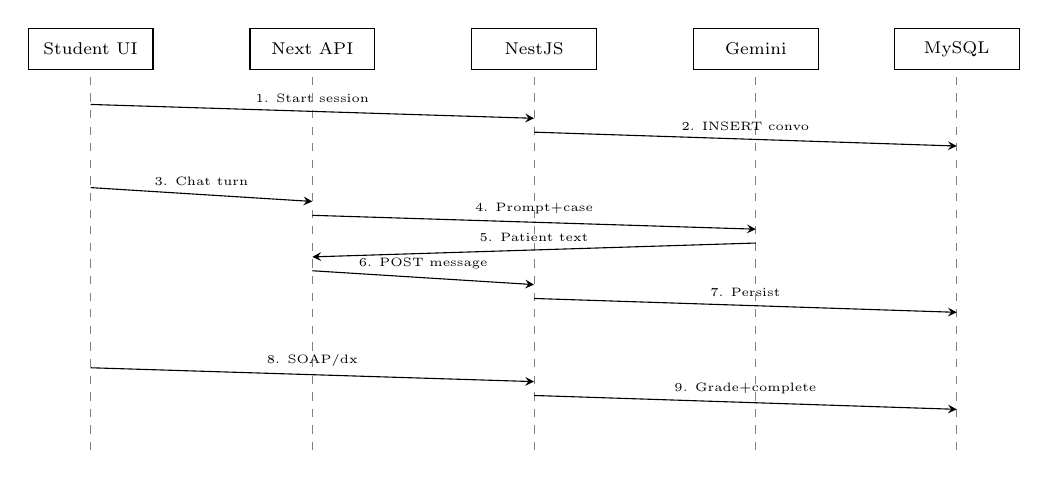
\begin{tikzpicture}[
    scale=0.88,
    transform shape,
    node distance=0.55cm,
    actor/.style={rectangle, draw, minimum width=1.8cm, minimum height=0.6cm, font=\scriptsize},
    msg/.style={->, >=stealth, font=\tiny},
    lifeline/.style={dashed, gray}
  ]
    \node[actor] (stu) at (0,0) {Student UI};
    \node[actor] (next) at (3.2,0) {Next API};
    \node[actor] (nest) at (6.4,0) {NestJS};
    \node[actor] (llm) at (9.6,0) {Gemini};
    \node[actor] (db) at (12.5,0) {MySQL};
    \foreach \x in {0,3.2,6.4,9.6,12.5} {
      \draw[lifeline] (\x,-0.4) -- (\x,-5.8);
    }
    \draw[msg] (0,-0.8) -- node[above] {1. Start session} (6.4,-1.0);
    \draw[msg] (6.4,-1.2) -- node[above] {2. INSERT convo} (12.5,-1.4);
    \draw[msg] (0,-2.0) -- node[above] {3. Chat turn} (3.2,-2.2);
    \draw[msg] (3.2,-2.4) -- node[above] {4. Prompt+case} (9.6,-2.6);
    \draw[msg] (9.6,-2.8) -- node[above] {5. Patient text} (3.2,-3.0);
    \draw[msg] (3.2,-3.2) -- node[above] {6. POST message} (6.4,-3.4);
    \draw[msg] (6.4,-3.6) -- node[above] {7. Persist} (12.5,-3.8);
    \draw[msg] (0,-4.6) -- node[above] {8. SOAP/dx} (6.4,-4.8);
    \draw[msg] (6.4,-5.0) -- node[above] {9. Grade+complete} (12.5,-5.2);
  \end{tikzpicture}
  \caption{Sequence of operations for a single MedPrep encounter turn (simplified).}
  \label{fig:medprep-sequence}
\end{figure}
